\documentclass{article}

\usepackage[dutch]{babel}
\usepackage[margin=3cm]{geometry}
\usepackage{graphicx}
\usepackage{float}
\usepackage{caption}
\usepackage{hyperref}
\usepackage{amsmath}
\usepackage{wrapfig}
\usepackage[parfill]{parskip}
\usepackage{listings}
\usepackage{xcolor}
\usepackage{gensymb}

\lstset{
basicstyle=\ttfamily,
frame=single,
breakatwhitespace=false,         % sets if automatic breaks should only happen at whitespace
breaklines=true,                 % sets automatic line breaking
commentstyle=\color{blue},
showstringspaces=false
}

% fonts
\usepackage[T1]{fontenc}
\usepackage{helvet}
\renewcommand{\familydefault}{\sfdefault}
 
\graphicspath{{img/}} 

\newcommand{\bold}[1]{\textbf{#1}}

\begin{document}

\begin{titlepage}
    \author{Tuur Vanhoutte}
    \title{Sensors \& Interfacing: labo}
\end{titlepage}

\pagenumbering{gobble}
\maketitle
\newpage
\tableofcontents
\newpage

\pagenumbering{arabic}

\section{One-wire bus}
\begin{itemize}
    \item Ontworpen om over lange afstanden kleine hoeveelheden data te sturen. 
    \item Kan makkelijk in kleine, goedkope sensoren ingebouwd worden
    \item Voorzien van 3 pootjes (3 draden): 2 voor voeding (+ en -), 1 voor data
    \item 1 master en 1 of meerdere slaves, elke slave heeft een uniek 64bit adres of slave ID
\end{itemize}




\subsection{Schema}

\begin{figure}[H]
    \centering
    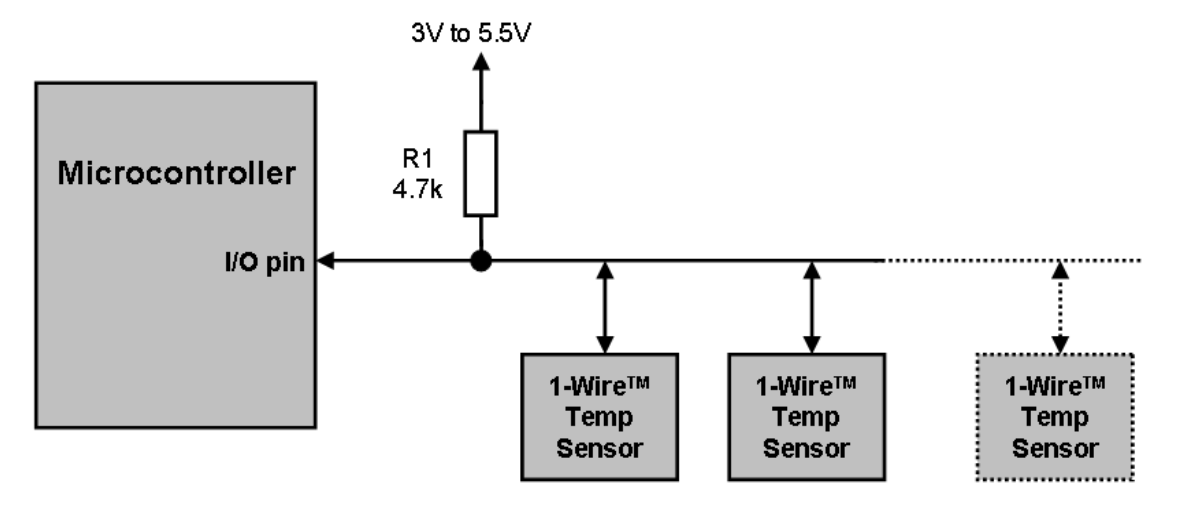
\includegraphics[width=0.5\textwidth]{Screenshot_20200619_150049.png}
    \caption{Schema 1-wire bus met meerdere slaves}
\end{figure}

\subsection{Timingdiagram}
Omdat er maar 1 draad beschikbaar is voor communicatie, moet het protocol vertrouwen op erg strikte timing.
Raspbian voorziet een driver die daarvoor zorgt.

\begin{figure}[H]
    \centering
    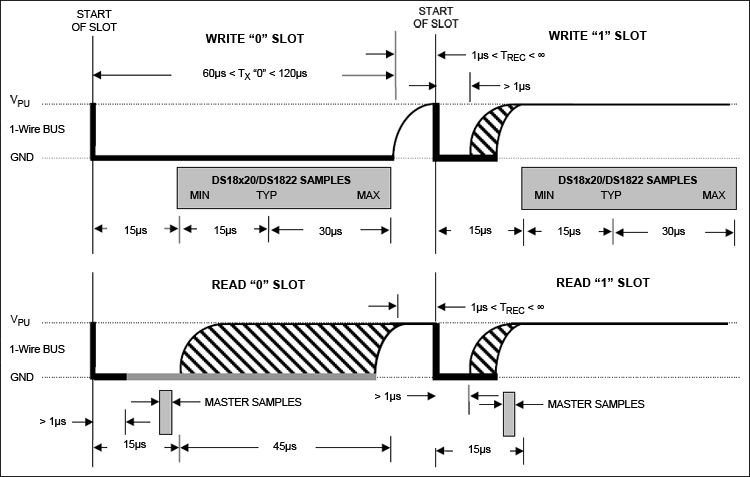
\includegraphics[width=0.5\textwidth]{timing-1w.png}
    \caption{Timingdiagram}
\end{figure}

\subsection{Werking}
\subsubsection{Open-collector outputs}
Het is niet mogelijk om zomaar een digitale 0 voor te stellen als 0V, en een digitale 1 als 3.3V.
Dat kan zorgen voor kortsluiting. Daarom gebruiken we een open-collector uitgang:

\begin{figure}[H]
    \centering
    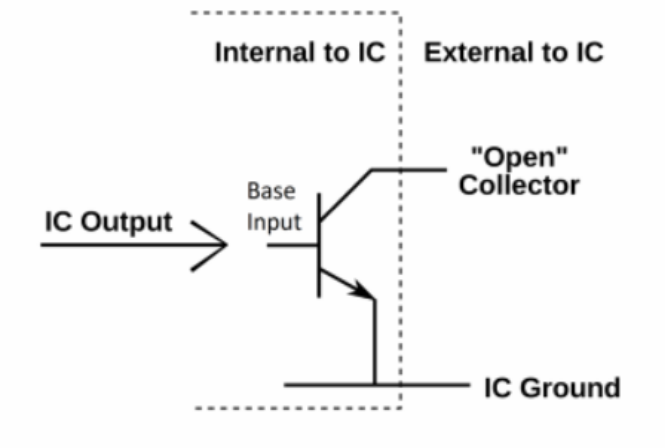
\includegraphics[width=0.5\textwidth]{open-collector.png}
    \caption{Interne schakeling van een open-collector uitgang}
\end{figure}

In plaats van slaves toe te laten zelf een spanning op de bus te leggen, brengen we hem standaard op
een hoog signaalniveau d.m.v. een \bold{externe pull-up weerstand}. 
De uitgangen van ICs die op de bus communiceren worden dan voorzien van een \bold{extra transistor}
waarvan de emitter (of source bij een FET) verbonden is met massa. 
De basis (of gate) is verbonden met de uitgang van de logica en de collector (of drain)
met de uitgangspin en dus de bus.

\subsubsection{Data verzenden}
De bus wordt via een externe weerstand verbonden met de voedingsspanning.
Aangesloten apparaten in rust kunnen we beschouwen als een open circuit (de uitgangstransistor geleidt niet).
De bus blijft dus standaard op een hoog signaalniveau en er vloeit (in theorie) geen stroom.

Om data te verzenden, kan een deelnemer de transistor in geleiding brengen en zo de bus verbinden met
massa. Op dit moment zal er een stroom vloeien, door de pull-up weerstand en uitgangstransistor naar massa. 
De spanning op de bus bedraagt op dat moment (bijna) 0V, gegeven door de spanningsdeler tussen de 
externe pull-up weerstand en de restweerstand van de transistor in geleiding.

\begin{figure}[H]
    \centering
    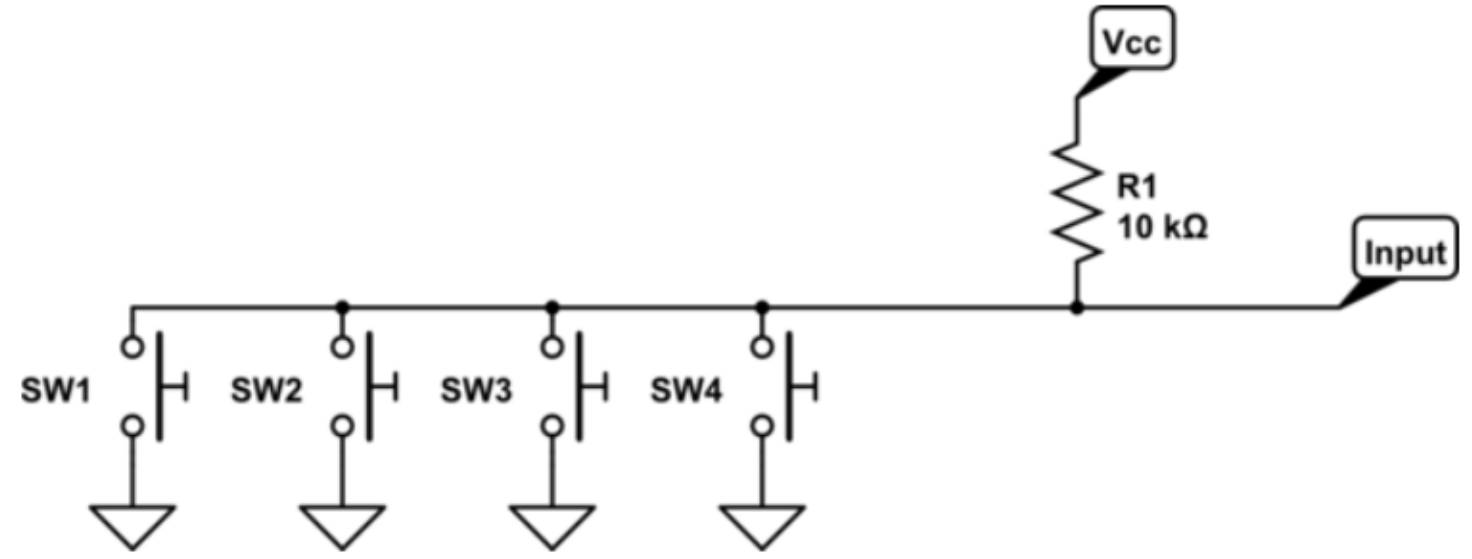
\includegraphics[width=0.5\textwidth]{Screenshot_20200619_152619.png}
    \caption{Meerdere open-collector outputs (hier voorgesteld door schakelaars), op dezelfde bus}
\end{figure}

Wanneer nu een andere deelnemer op hetzelfde moment gaat communiceren, kan ook die enkel een
verbinding van de bus naar massa maken. Elektrisch vormt dit geen enkel probleem, maar de communicatie
van beide deelnemers zal uiteraard nog steeds verstoord zijn.


\subsection{Voordelen en nadalen}
\subsubsection{Voordelen}
\begin{itemize}
    \item \bold{Geen elektrische conflicten}: Meerdere deelnemers kunnen enkel meerdere verbindingen naar massa maken.
    \item \bold{Flexibele spanning}: Omdat enkel de uitgangstransistor elektrisch met de bus verbonden is, is het
    makkelijk om chips te maken die een verschillende spanning op de bus t.o.v. hun voedingsspanning
    kunnen tolereren.
\end{itemize}

\subsubsection{Nadelen}
\begin{itemize}
    \item \bold{Hoog stroomverbruik}: Een laag signaalniveau betekent een constante stroom door de geleider, en ook
    bij hoog signaalniveau zal er nog een kleine lekstroom door de transistors vloeien.
\end{itemize}

\section{Bitoperaties events}
\subsection{Bits \& bytes}
\begin{figure}[H]
    \centering
    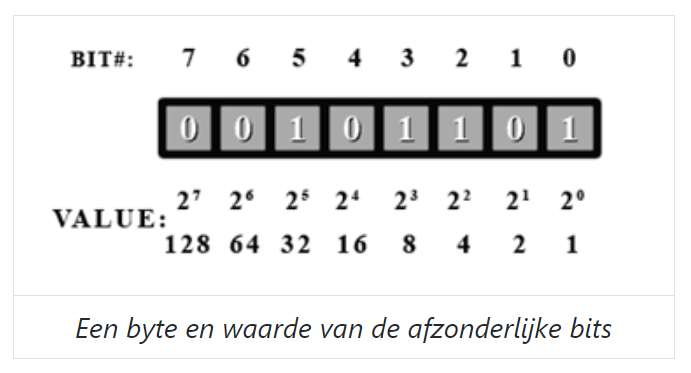
\includegraphics[width=0.5\textwidth]{bits.png}
    \caption{1 byte. Least Significant Bit (LSB) = rechts, Most Significant Bit (MSB) = links}
\end{figure}

\subsubsection{Hexadecimale notatie}
\begin{figure}[H]
    \centering
    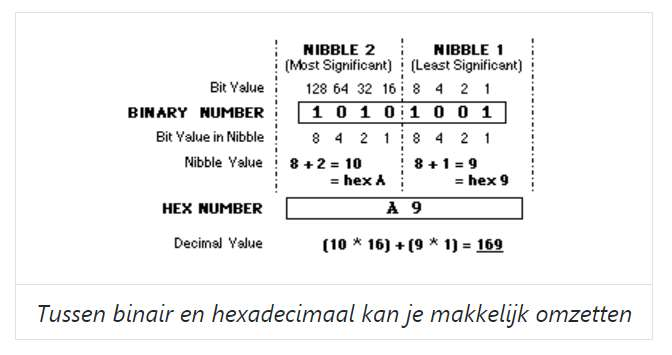
\includegraphics[width=0.7\textwidth]{hexa.png}
    \caption{Omzetting van binair naar hexadecimaal. 1 nibble = 4 bits}
\end{figure}

\subsection{Python}
\begin{itemize}
    \item bin(x) om waarden om te zetten naar binair
    \item hex(x) om waarden om te zetten naar hexadecimaal
    \item int(x) om waarden om te zetten naar decimaal
    \item ord('a') om chars om te zetten naar hexadecimaal
\end{itemize}

\subsection{Bitwise Operators}
\begin{itemize}
    \item And: als beide inputs == 1, output = 1, anders 0
    \item Or: als 1 van de inputs == 1, output 1, anders 0
    \item Not: draai input om: 1 wordt 0, 0 wordt 1
    \item Xor: als precies 1 van de inputs == 1, output = 1, anders 0
\end{itemize}

\begin{table}[H]
\begin{tabular}{|l|l|}
\hline
\multicolumn{1}{|c|}{\textbf{Bitwise operator}} & \multicolumn{1}{c|}{\textbf{Symbol in python}} \\ \hline
and                                             & \&                                             \\ \hline
or                                              & |                                              \\ \hline
not                                             & $\sim$                                         \\ \hline
xor                                             & \textasciicircum{}                             \\ \hline
\end{tabular}
\end{table}

\begin{figure}[H]
    \centering
    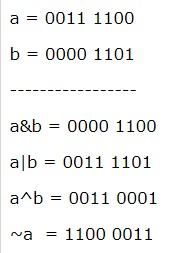
\includegraphics[width=0.25\textwidth]{bitoperator-examples.png}
    \caption{Voorbeelden bitoperaties}
\end{figure}

\subsubsection{Set bits}
De OR-operatie kan je gebruiken om bits aan te zetten, ongeacht hun huidige waarde:
\begin{lstlisting}[language=Python]
>>> have = 0b11001010 # het register nu 
>>> mask = 0b00000100 # dus maak ik een getal waar ENKEL bit 2 "aan" is
>>> xxxx = 0b11001110 # wat ik wil nu wil uitkomen

# en ik gebruik dat met de |-operator om de bit "aan" te zetten
>>> result = have | mask 
>>> xxxx == result
True 
\end{lstlisting}

Hetzelfde principe kan je gebruiken met de \&-operator om bits op 0 te zetten,
of bits te filteren (stel dat je alleen bit 2 nodig hebt, dan is je masker 0b00000100)

\subsubsection{Toggle bits}
Togglen van een bit kan je doen met de XOR-operatie (\textasciicircum{})

\subsubsection{Bitwise NOT}
Het resultaat van de NOT-operatie op een binair getal is niet het omgekeerde van het getal, 
maar het negatieve getal. Om dat op te lossen moet je het negatieve getal AND-en met 0xFF.

\subsubsection{Shift left/right}
We kunnen bits opschuiven met $<<$ en $>>$. Dit is hetzelfde als vermenigvuldigen met 2 en delen met 2.

\begin{lstlisting}[language=Python]
>>> 0b00010100 >> 4 == 0b00000001
True
>>> 0b11001010 << 4 == 0b110010100000
True
>>> 0b11001010 << 8 == 0b1100101000000000
True
\end{lstlisting}

\subsubsection{In-place operators}
\begin{lstlisting}[language=Python]
>>> x += 2       # x = x + 2
>>> x -= 2       # x = x - 2
>>> x |= 4       # x = x | 0x04 --> bit 2 is nu 1
>>> x &= 253     # x = x & 0xfd --> bit 1 is nu 0
>>> x ^= 0xf0    # x = x ^ 0xf0 --> 4 MSB worden getoggled
>>> x <<= 2      # x = x << 2 --> alle bits 2 plaatsen naar links
>>> x >>= 3      # x = x >> 3 --> alle bits 3 plaatsen naar rechts
\end{lstlisting}

\subsubsection{Volgorde van bewerkingen}
\begin{enumerate}
    \item not $\sim$
    \item shift $<<$, $>>$
    \item and \&
    \item xor \textasciicircum{}
    \item or |
\end{enumerate}

Gebruik haakjes!

\subsection{Binary Coded Decimals (BCD)}
Bij BCD worden 4 bits gebruikt om 1 decimaal cijfer weer te geven

Voor het getal 91 worden dus groepjes van 4 bits gebruikt om elk getal weer te geven:
\begin{lstlisting}
Decimal:       9     1
Binary:     1001  0001
\end{lstlisting}

\bold{Opgelet}: je mag niet zomaar wiskundige operaties toepassen op een BCD code.
De decimale waarde van BCD-getal 91 is 128+32+1 = 161

\subsection{Interrupts \& Events}
\subsubsection{Interrupts}
Een interrupt is een voorziening om de processor op de hoogte te stellen van een bepaalde
gebeurtenis. 
De CPU zal daarop zijn huidige werk onderbreken en een Interrupt Service Routine (ISR),
ook wel Interrupt Handler genoemd, uitvoeren. 

Na afloop gaat hij weer verder met de taak waar hij
voordien aan werkte. Op deze manier hoeft er geen CPU-power verspild te worden met het
wachten op gebeurtenissen.

\subsubsection{Events}
= signaalovergang

\begin{lstlisting}[language=Python]
GPIO.add_event_detect(channel, GPIO.RISING) # add rising edge detection

do_something_else() # thread is bezig met andere dingen

if GPIO.event_detected(channel):
    print('Button released')
    # dit werkt nog altijd
\end{lstlisting}


\subsubsection{Callbacks}
\begin{lstlisting}[language=Python]
def my_callback(channel):
    print('This is a edge event callback function!')
    print('Edge detected on channel %s'%channel)
    print('This is run in a different thread to your main program')

GPIO.add_event_detect(channel, GPIO.RISING, callback=my_callback)
\end{lstlisting}

Je kan meerdere callbacks op eenzelfde pin registeren door gewoon meerdere keren de methode GPIO.add\_event\_callback(\dots) op te roepen.

\bold{Bouncetime}

Bijkomende parameter bij add\_event\_detect(): aantal milliseconden dat dient om de knop te ontdenderen (debounce). 


\section{Seriele communcatie}
Bv: communicatie tussen Arduino en Raspberry Pi. 

\bold{Opgelet:} de Pi werkt op 3.3V en de meeste arduino's op 5V. 
We moeten een levelshifter gebruiken.

\subsection{Serieel protocol}
Zeer eenvoudig om full-duplex te werken:

\begin{itemize}
    \item een draad om data te versturen
    \item een draad om data te ontvangen
    \item gemeenschappelijke massa (GND)
    \item Het is een point-to-point verbinding: 2 deelnemers, dus geen adressering nodig
\end{itemize}

De chip die zo'n seriele interface aanstuurt noemt men een UART (Universal Asynchronous Receiver / Transmitter).
De termen UART, RS-232 en seriele poort worden vaak door elkaar gebruikt. RS-232 of Recommended Standard 232
omschrijft connectoren, elektrische eigenschappen \dots

\subsection{Hardware (Layer 1)}
\begin{itemize}
    \item Oorspronkelijk:
    \begin{itemize}
        \item 0 = 3 tot 15V
        \item 1 = -3 tot -15V
    \end{itemize}
    \item Tegenwoordig:
    \begin{itemize}
        \item Veel devices werken op -5V tot +5V
        \item Hetzelfde protocol maar op TTL-niveau (0-5V)
    \end{itemize}
    \item De bus is standaard hoog, wat door de UART zelf geregeld wordt. We moeten dus geen pull-up voorzien.
\end{itemize}

\begin{figure}[H]
    \centering
    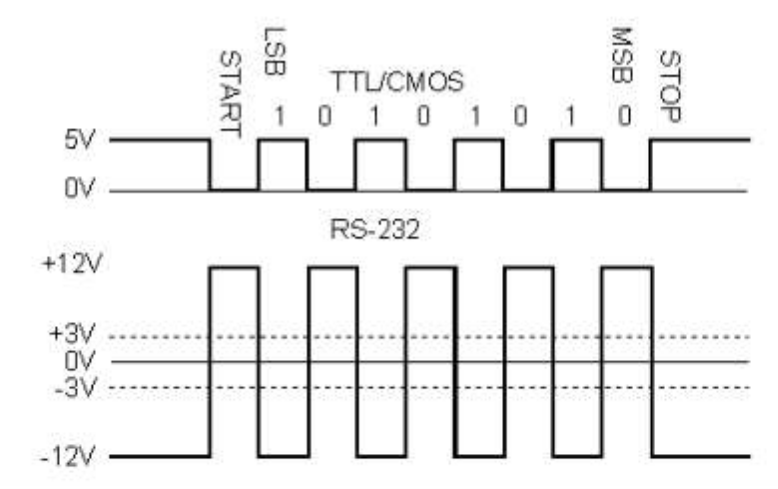
\includegraphics[width=0.4\textwidth]{ttl-vs-rs232.png}
    \caption{TTL (boven) vs RS-232 (onder)}
\end{figure}

\subsubsection{Crossed cable of null-modemkabel}
De TX-pin van de zender moet verbonden worden met de RX-pin van de ontvanger en vice versa. 
In de context van de oude seriele poort noemt men zo'n crossed cable een null-modemkabel.

Seriële verbindingen werden veel gebruikt voor het verbinden van een modem met je PC, en met zo’n null-modemkabel kon je dan 2 computers rechtstreeks
verbinden zonder een modem tussen.

\subsection{Protocol (Layer 2)}
Alle data bits bevinden zich tussen een start- en stopsignaal. De start bit is één 0-bit, de volgende
zeven of acht bits vormen een databyte. Eventueel kan er als controle nog een parity bit worden
toegevoegd. Het teken wordt telkens afgesloten door één of twee stop bits.

Aan de kant van de ontvanger wordt de data aan het start- en stopsignaal herkend.
Het aantal start-, data- en stopbits kan worden ingesteld en moet uiteraard langs beide kanten overeen komen.

\subsubsection{Baudrate}
= De snelheid = symbolen per seconde

\begin{itemize}
    \item Zender en ontvanger moeten dezelfde baudrate hebben
    \item Hogere rate $\rightarrow$ hogere eisen qua elektrische verbinding en timingnauwkeurigheid
    \item Lagere rate $\rightarrow$ minder snelle communicatie, maar grotere maximale kabellengte
    \item Positieve spanning: lage bit, negatieve spanning: hoge bit
\end{itemize}

\bold{Veelgebruikte baudrates:}
\begin{itemize}
    \item 9600 baud (=veelvoud van 300, vandaag standaard maar traag, wordt door vrijwel elke UART ondersteund)
    \item 19200, 57600, 115200 baud (= veelvouden van 9600)
    \item 64k baud en veelvouden
    \item 1M baud en veelvouden
\end{itemize}

\begin{figure}[H]
    \centering
    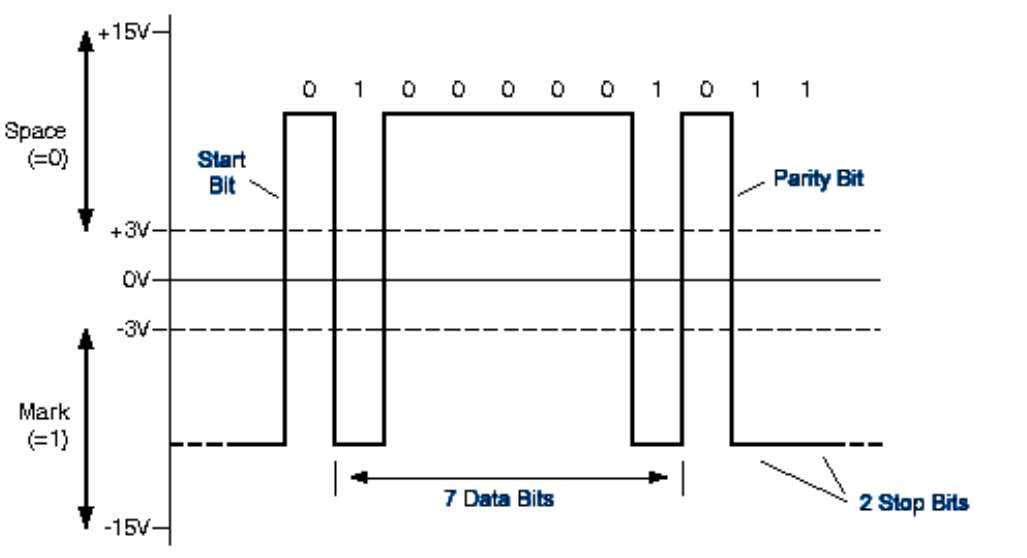
\includegraphics[width=0.5\textwidth]{serielecommunicatie.png}
    \caption{Timingdiagram seriele communicatie}
\end{figure}

\subsection{Flow control}
Mechanisme waarmee zender en ontvanger elkaar kunnen verwittigen wanneer ze klaar zijn voor datatransmissie. 
Dat kan zowel in hardware (dus met extra signaaldraden), of in software met speciale karakters.

\bold{Hardware:}
\begin{itemize}
    \item RTS/CTS: Request To Send/Clear To Send pins worden gebruikt om aan te geven dat het apparaat klaar is om data te sturen/ontvangen
    \item DSR/DTR: Data Set Ready/Data Terminal Ready-lijnen die eigenlijk aangeven dat het apparaat online en klaar is, worden soms misbruikt voor flow control
\end{itemize}

\bold{Software:}
\begin{itemize}
    \item XON/XOFF: Zijn speciale ASCII-controletekens die als data van ontvanger naar verzender worden gestuurd om transmissie te starten/stoppen
\end{itemize}

Flow control was van groot belang om een modem aan te sluiten maar wordt vandaag niet meer veel gebruikt.

\subsection{Verschillende opties seriele communicatie}
\begin{enumerate}
    \item USB kabel
    \item Gebruik van seriele pins op de GPIO connector
\end{enumerate}

\subsection{Byte serieel versturen}
Het serieel protocol heeft maar 1 draad om een byte (char) te versturen of ontvangen.
Daarom moeten we elke byte ontleden en bit per bit versturen. De meeste protocollen starten met de MSB (meest linkse bit).

\subsubsection{In python: PySerial}
= een library om makkelijk een seriele poort te openen:

\begin{lstlisting}[language=Python]
import serial
ser = serial.Serial('/dev/ttyS0') # open serial port
print(ser.name)                   # check which port was really used
ser.write(b'hello')               # write a string
ser.close()                       # close port
\end{lstlisting}

\begin{lstlisting}[language=Python]
from serial import Serial, PARITY_NONE

# simple echo server
with Serial('/dev/ttyS0', 115200, bytesize=8, parity=PARITY_NONE, stopbits=1) as port:
    while True:
        line = port.readline()
        port.write(line)
\end{lstlisting}

\subsection{Level shifter}
= een module die we kunnen gebruiken om componenten die op een verschillende 
spanning werken digitaal met elkaar te verbinden. 

\begin{itemize}
    \item De ene kant is low voltage (LV), de andere high voltage (HV)
\end{itemize}

\begin{figure}[H]
    \centering
    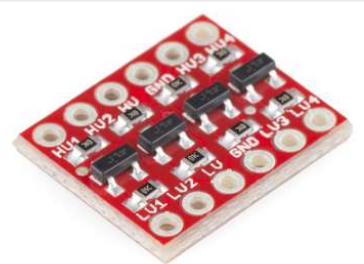
\includegraphics[width=0.2\textwidth]{levelshifter.png}
    \caption{Een levelshifter met 4 bits}
\end{figure}

\begin{figure}[H]
    \centering
    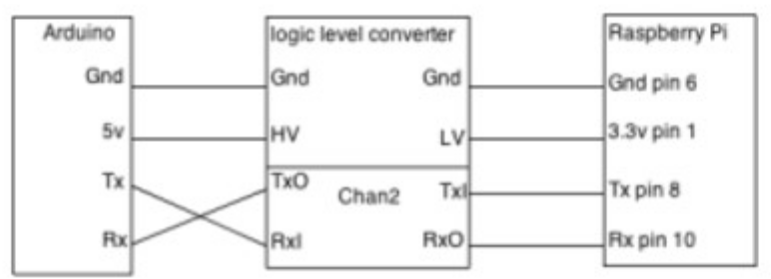
\includegraphics[width=0.4\textwidth]{levelshifter-arduino.png}
    \caption{Verbinding tussen Arduino en Pi. Let op de crossed cabling tussen Arduino en levelshifter}
\end{figure}

\section{Shiftregister}
Een shiftregister ontvangt een aantal bits in serie die parallel naar buiten gebracht worden. 
Op die manier kunnen we via één data pin van onze raspberry pi meerdere uitgangen creëren.

Een shiftregister is opgebouwd uit een aantal elektronische componenten (flip flops of latches) die in serie
geschakeld worden met elkaar en dezelfde klok delen. De uitgang van elke flip flop wordt gebruikt als ingang van de volgende. Zo’n schakelingen wordt ook een
cascade (waterval) schakeling genoemd. Op die manier kan je ook meerdere shift registers met elkaar
verbinden.

\subsection{Shiftregister 74HC595}
De 74HC595 is een high speed 8-bit `serieel in parallel out' shiftregister.
We kunnen dus 8 bits na elkaar serieel versturen naar het register, 
die bits worden vervolgens naar 8 parallelle uitgangen gebracht.

Dit shiftregister heeft ook een storage register dat de data bij kan houden. 
Voor het 7-segment display is dit handig omdat we de vorige waarde kunnen blijven tonen.

\subsection{Pinnummering}

\begin{figure}[H]
    \centering
    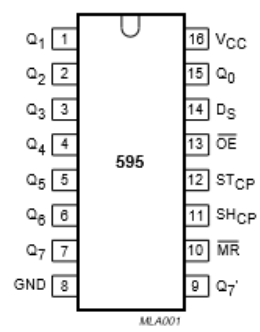
\includegraphics[width=0.3\textwidth]{shiftregister-pins.png}
    \caption{Pin configuratie 74HC595}
\end{figure}

Deze pins moeten we verbinden met een GPIO-pin van de RPi:
\begin{itemize}
    \item Master Reset (MR)
    \item De twee klokken (SHCP en STCP)
    \item De Output Enable (OE)
    \item De Serial Data (SD of $\text{D}_{\text{S}}$)
\end{itemize}

Q0 t.e.m. Q7 sluiten we aan ons component (hier: 7-segment display)

Door gebruik te maken van 5 GPIO pinnen beschikken we nu over 8 digitale uitgangen.
Door een shiftregister toe te voegen beschikken we over 16 uitgangen met onze 5 GPIO-pinnen.

\subsection{Protocol}

\begin{figure}[H]
    \centering
    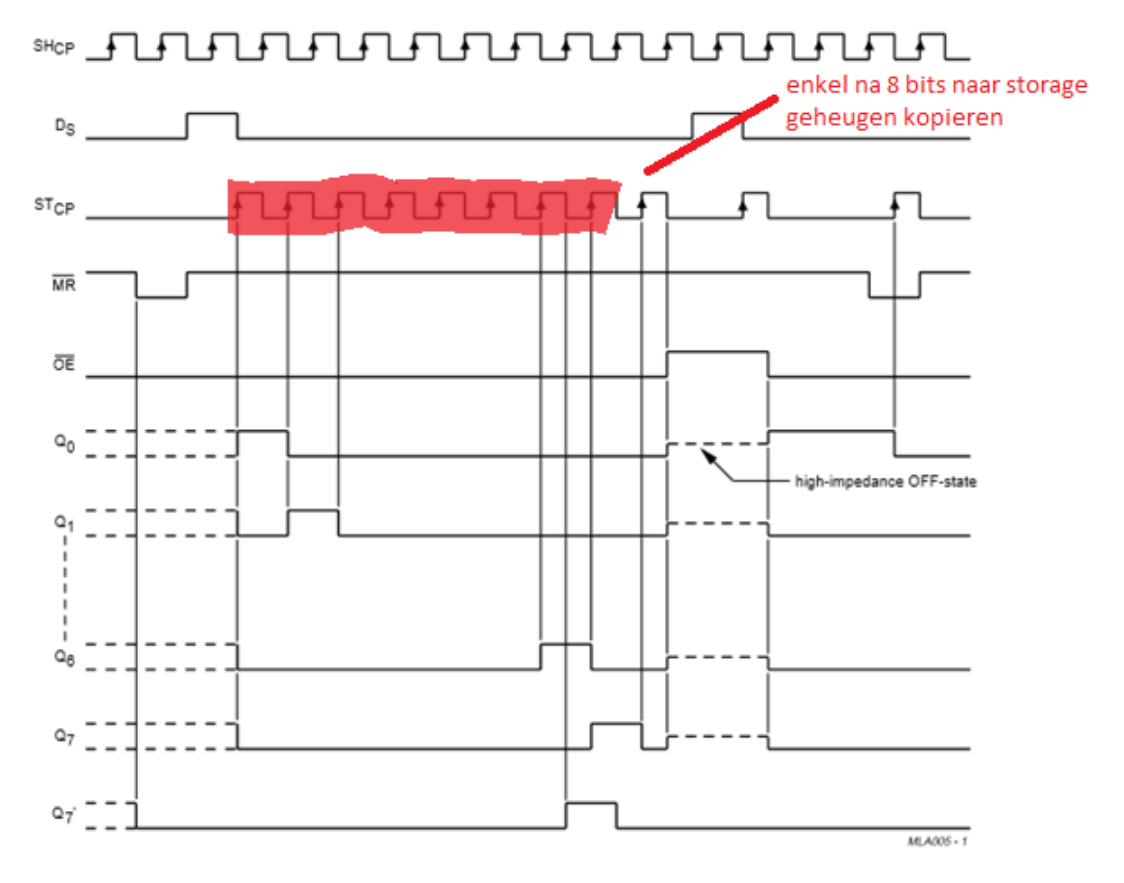
\includegraphics[width=0.8\textwidth]{timing-shift.png}
    \caption{Timingdiagram shiftregister 74HC595}
\end{figure}


\subsection{7-segment display met shiftregister}
= display dat bestaat uit 8 segmenten (7 voor het cijfer + 1 voor het punt)

\subsubsection{Twee soorten}
\begin{enumerate}
    \item Common Cathode
    \item Common Anode
\end{enumerate}

\begin{figure}[H]
    \centering
    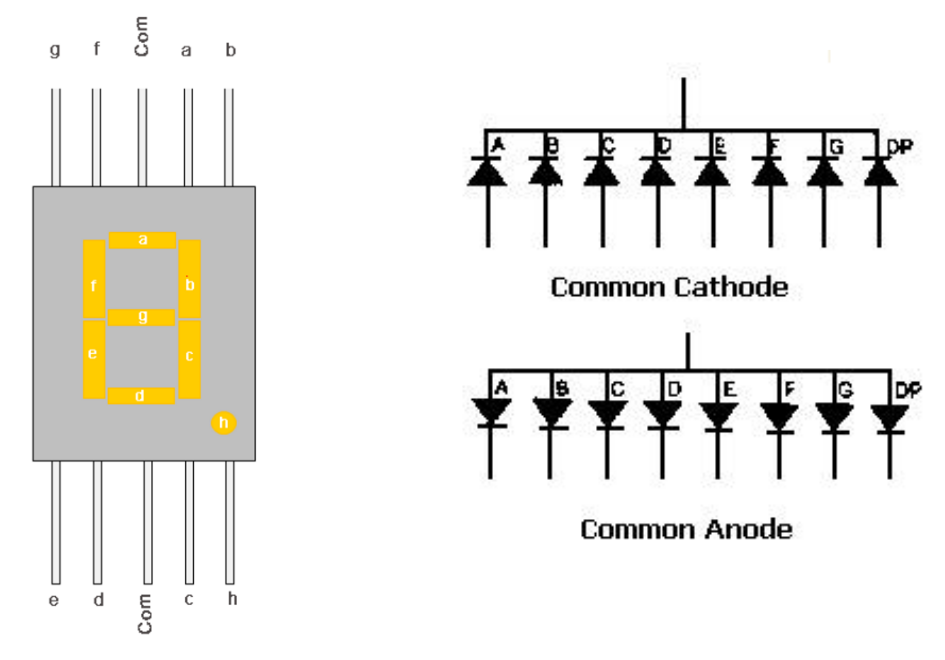
\includegraphics[width=0.45\textwidth]{7-display.png}
    \caption{7-segment display: twee soorten}
\end{figure}

\begin{figure}[H]
    \centering
    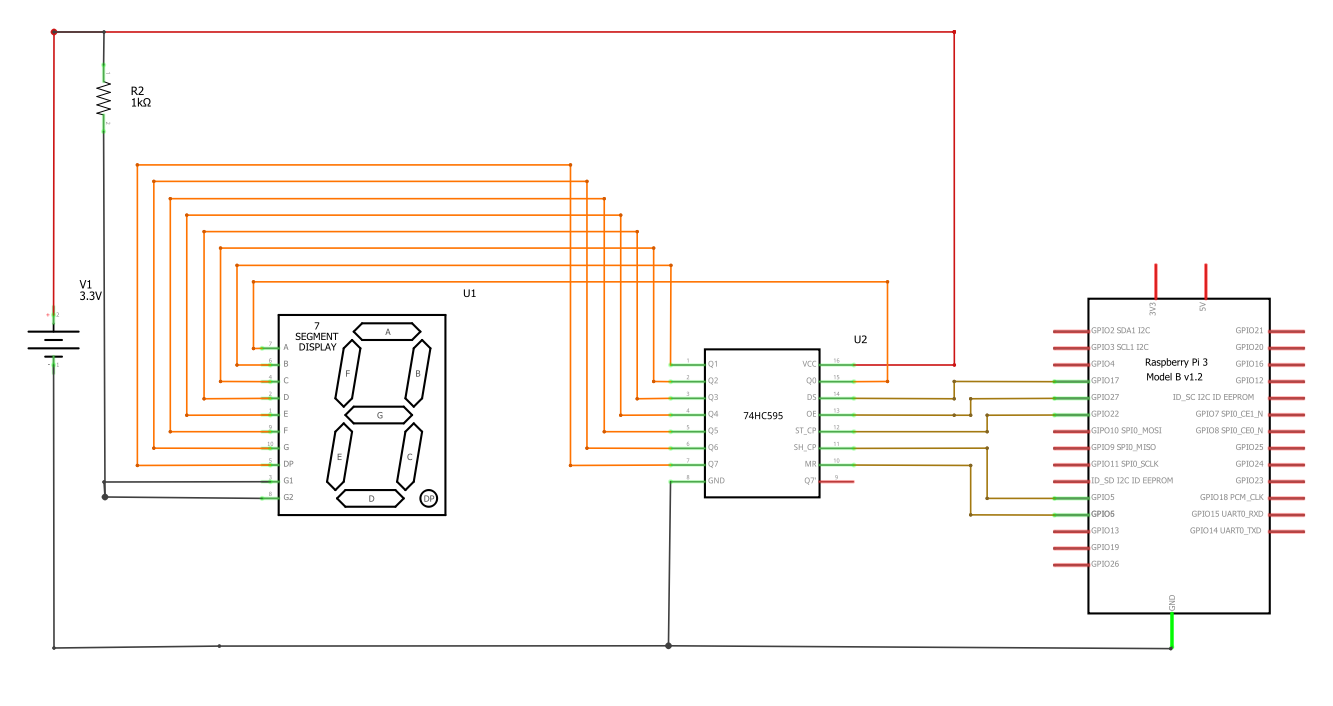
\includegraphics[width=\textwidth]{shiftregister-7-segment.png}
    \caption{7 segment display (common anode) met 74HC595}
\end{figure}

\subsection{Cascade schakeling van shiftregisters}

De kloklijnen en de OE en MR worden parallel verbonden met het volgend shiftregister. 
De laatste bit, die in principe zou wegvallen, wordt na een puls op de SHCP ter beschikking gesteld op de uitgang Q7’. 
De uitgang Q7’ wordt aangesloten op de DS van het tweede register.

\begin{figure}[H]
    \centering
    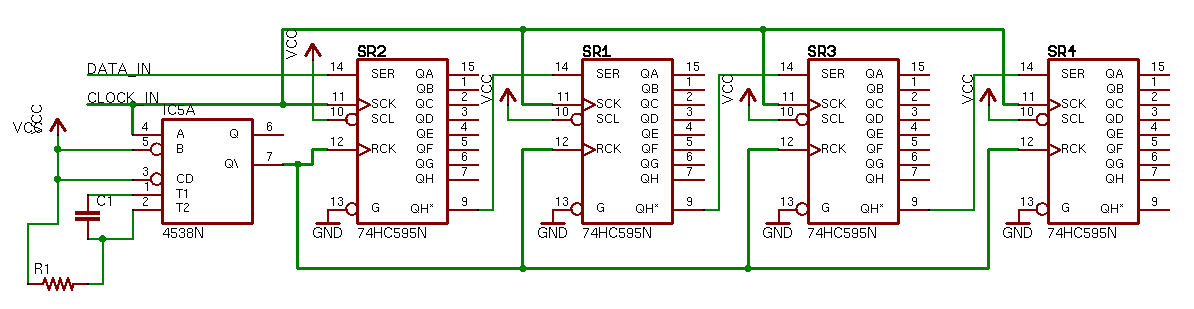
\includegraphics[width=\textwidth]{shiftregister-4cascade.png}
    \caption{4 shiftregisters in cascade geschakeld}
\end{figure}


\subsection{Shift input}
Sommige shiftregisters kunnen ook als input gebruikt worden $\rightarrow$ meerdere digitale inputs met slechts 5 pinnen.


\section{Analoge ingangen}

\subsection{Principe analoog naar digitaal omvormer}
= omvormen van een analoog signaal (spanningswaarden) naar een digitaal signaal (0 en 1)

Voor een digitale ingang hebben we maar 1 bit nodig in het computergeheugen (bv: de knop is wel of niet ingedrukt)

Voor een analoge ingang hebben we zo veel mogelijk tussenstappen nodig om het analoge signaal na te bootsen.
In onderstaande figuur hebben we een analoog signaal met 3 bits resolutie. 

\begin{figure}[H]
    \centering
    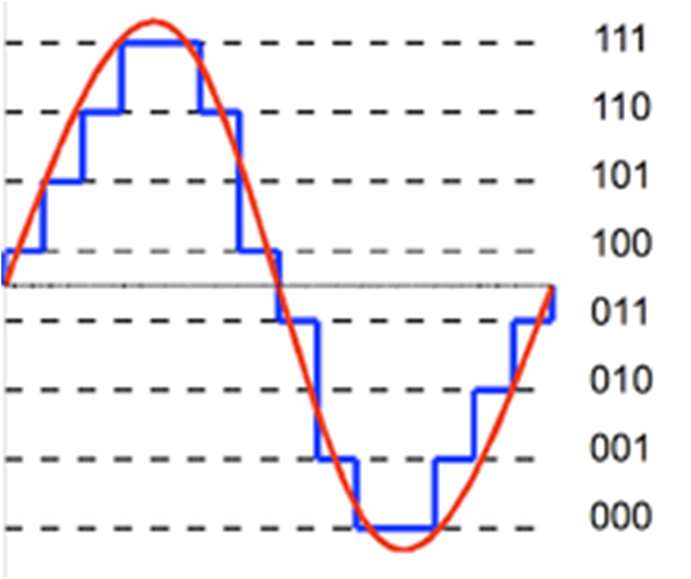
\includegraphics[width=0.3\textwidth]{analoge-ingangen.png}
    \caption{Voorbeeld analoog signaal met 3 bits resolutie $\rightarrow 2^3 = 8$}
\end{figure}

Onze MCP3004/3008 beschikt over 10 bits analoge ingangen = 1024 tussenstappen. 
Spanningsnauwkeurigheid: $\frac{3.3V}{1024} = 3.2mV$

\subsection{Serial Peripheral Interface (SPI)}
= een synchrone seriële interface tussen ten minste twee devices. 

\begin{itemize}
    \item Er is altijd één master en \bold{ten minste één} slave. De master regelt de communicatie. 
    \item Synchroon betekent dat de klokken van de verschillende devices worden gesynchroniseerd of gelijkgesteld met elkaar via een externe klok of een signaal van de master. 
    \item Serieel houdt in dat de data na elkaar wordt verstuurd.
    \item De communicatie is full-duplex
    \item 4-draadse seriele bus
\end{itemize}

De 4 gebruikte lijnen:
\begin{itemize}
    \item SCLK (Serial Clock)
    \item MOSI (Master Output Slave Input)
    \item MISO (Master Input Slave Output)
    \item SS (Slave Select), active low, wordt soms aangeduid met CE (Chip Enable) of CS (Chip Select)
\end{itemize}

\begin{figure}[H]
    \centering
    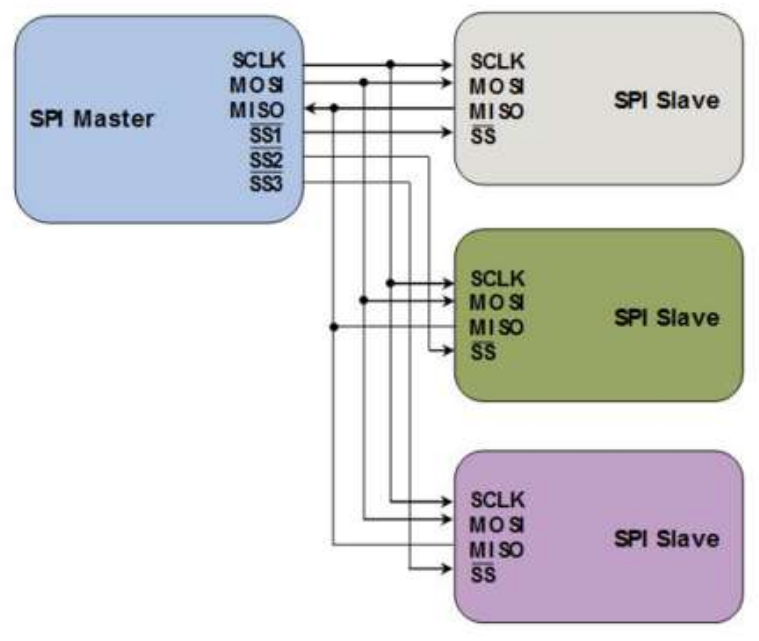
\includegraphics[width=0.4\textwidth]{spi.png}
    \caption{SPI master met 3 slaves}
\end{figure}

De Raspberry Pi beschikt over 2 Slave Select pinnen, dus we kunnen 2 SPI slaves aansluiten.

\subsection{Logische werking MCP3004/3008}
= 4 of 8 kanaal 10-bit A/D-convertors met een SPI-interface.

We kunnen aan deze IC's 4 of 8 analoge sensoren aansluiten, de IC zet de analoge waarde om naar een 10-bits digitaal getal.
Via de SPI bus kunnen we de digitale data van de IC inlezen. 

\begin{figure}[H]
    \centering
    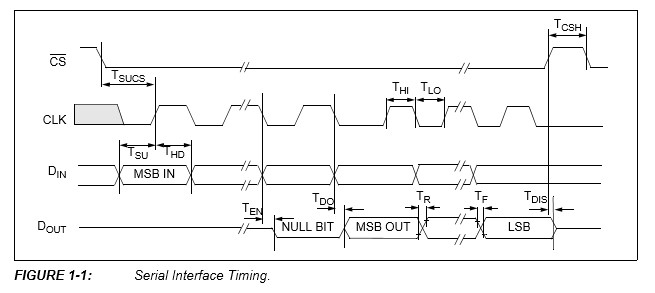
\includegraphics[width=0.7\textwidth]{timing-spi.png}
    \caption{SPI timingdiagram}
\end{figure}

Per databit die verstuurd wordt, moet de master (RPi) telkens een klok signaal genereren.
Tijdens de communicatie wordt de CS (=SS) naar een laag spanningsniveau gebracht

\subsubsection{Schakeling}

\begin{figure}[H]
    \centering
    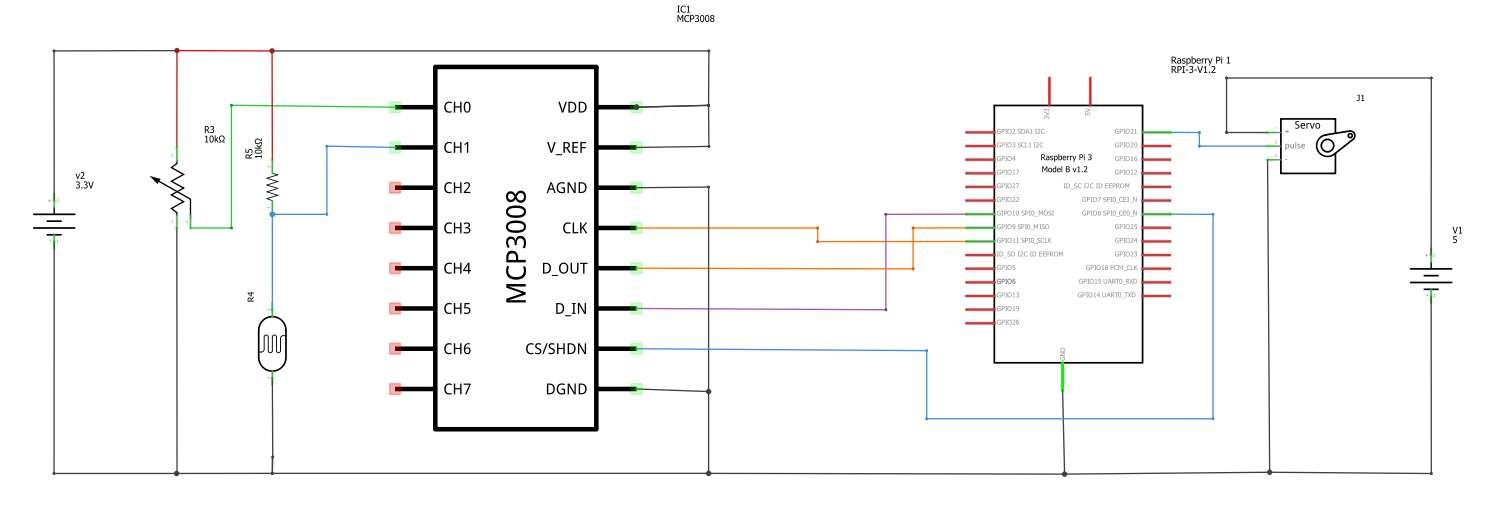
\includegraphics[width=\textwidth]{mcp.png}
    \caption{Schakeling MCP3008 met potentiometer en LDR}
\end{figure}


\subsubsection{Configuratie MCP3008}

Op de MCP3008 kan je het spanningsverschil tussen 2 kanalen opvragen ofwel een bepaalde spanning op een
analoog kanaal. Deze keuze kunnen we maken door de MSB op 1 (=single) of 0 (diff).

Het kanaal van de IC kan gekozen worden via de D2,D1 en D0 bit. 
Heb je een sensor aangesloten op CH3 dan moet je een 1011 meegeven. 
De MSB is 1 want we willen de spanning weten op het kanaal.

\subsubsection{Protocol MCP3008}

\begin{figure}[H]
    \centering
    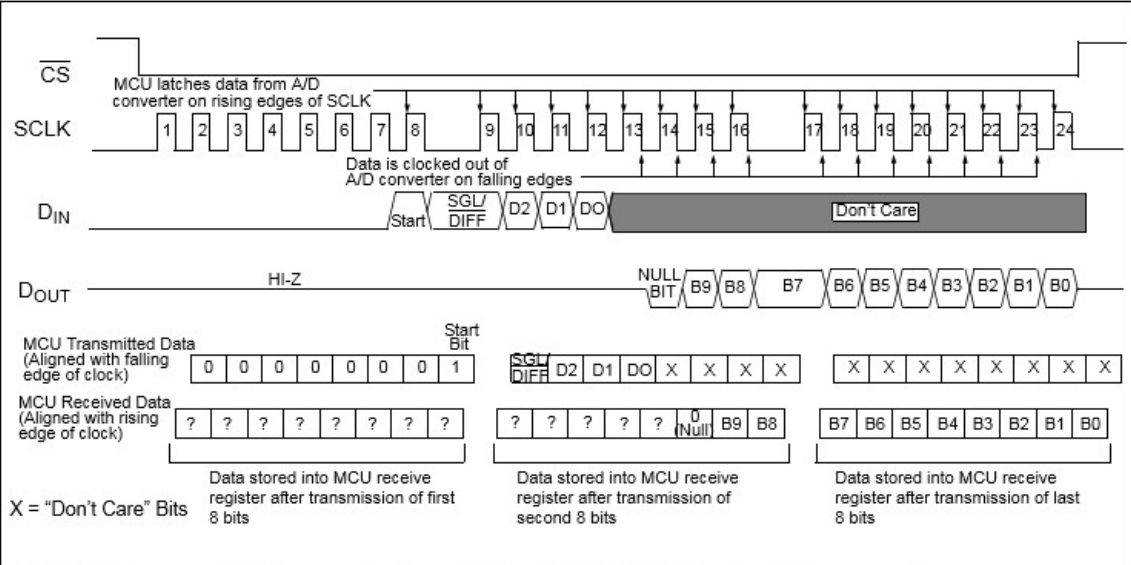
\includegraphics[width=0.75\textwidth]{timing-spi-mcp.png}
    \caption{SPI-communicatie met de MCP3004/3008}
\end{figure}

Communicatie met een slave:

\begin{itemize}
    \item Chip Select (CS) laag te brengen
    \item De master genereert een klokpuls (SCLK)
    \item Per tik van de klok kan er telkens een bit ontvangen en verstuurd worden.
    \item De $\text{D}_{\text{IN}}$ lijn is de data die we moeten versturen van de Pi naar de MCP.
    \item Er worden telkens 3 bytes verstuurd:
    \begin{enumerate}
        \item Byte met de startbit (0b00000001)
        \item Byte die de som is van Single/Diff en D2, D1 en D0. Deze bits moeten we 4 keer naar links schuiven
        \item Random byte (bv 0b00000000)
    \end{enumerate}
    \item En 3 bytes ontvangen:
    \begin{enumerate}
        \item Random byte 
        \item Byte 1: B9 en B8 van het binair getal, met $2^9=512$  en $2^8=256$
        \item Byte 2: de andere bits
    \end{enumerate}
\end{itemize}

\subsection{Python SpiDev}
= library om gemakkelijk SPI communicatie te doen

(zie week06-analoge-ingangen.pdf voor code)

\section{I2C}
= Inter-Integrated Circuit

\begin{itemize}
    \item Synchrone
    \item Multi-master/multi-slave 
    \item Tweedraads
    \begin{itemize}
        \item Kloksignaal (SCL) voor synchronisatie, met standaardfrequentie 100kHz
        \item Bidirectionele datalijn (SDA)
    \end{itemize}
    \item Serieel
    \item Slaves hebben 7-bit adressen
\end{itemize}

\subsection{I2C Protocol}
\begin{itemize}
    \item De bus is in rust hoog
    \item De master genereert een kloksignaal op SCL
    \item Een transmissie begint steeds met een startconditie en eindigt met een stopconditie.
    \item Kan zowel lezen als schrijven
    \item 1 datalijn $\rightarrow$ bit per bit versturen, startend bij de MSB
    \item Grote verschil met shiftregister: met I2C kunnen we rechtstreeks naar het correcte device sturen
    \item Het slave adres bestaat uit 7 bits + 1 R/W bit (=readen of writen, 1 = schrijven, 0 = lezen)
\end{itemize}

\begin{figure}[H]
    \centering
    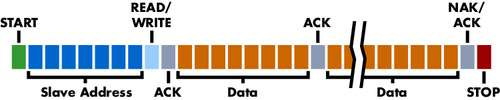
\includegraphics[width=0.75\textwidth]{i2c-protocol.png}
    \caption{I2C Protocol: start $\rightarrow$ adres + r/w $\rightarrow$ ack $\rightarrow$ data $\rightarrow$ ack $\rightarrow$ ... $\rightarrow$ ack $\rightarrow$ stop}
\end{figure}

\subsubsection{Start en stop condition}
De I2C bus is in rust toestand als beide lijnen (SCL en SDA) hoog zijn.

\begin{itemize}
    \item De startconditie is wanneer de SDA \bold{omlaag} getrokken wordt terwijl de kloklijn hoog staat.
    \item De stopconditie is wanneer de SDA \bold{omhoog} getrokken wordt terwijl de kloklijn hoog staat.
\end{itemize}

\begin{figure}[H]
    \centering
    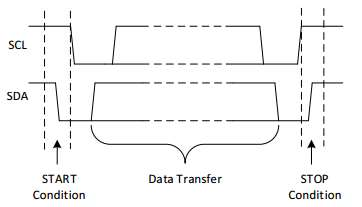
\includegraphics[width=0.5\textwidth]{i2c-start-stop.png}
    \caption{Start en stop}
\end{figure}

\subsubsection{Data transmission}
\begin{itemize}
    \item 1 byte serieel doorsturen (= bit per bit)
    \item Eerst de datalijn hoog of laag zetten, dan de klok hoog of laag zetten. 
    \item Zolang de klok hoog is, mag de data niet veranderen.
\end{itemize}

\begin{figure}[H]
    \centering
    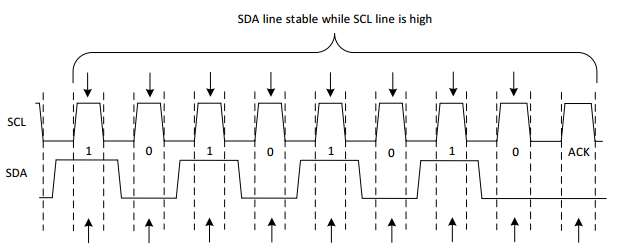
\includegraphics[width=0.5\textwidth]{i2c-timing.png}
    \caption{Timingdiagram I2C data}
\end{figure}

\subsubsection{Acknowledge}
Na elke byte kan de slave weergeven of hij de data al dan niet goed ontvangen heeft.

\subsection{PCF8574 I/O Expander for I2C bus}

\begin{figure}[H]
    \centering
    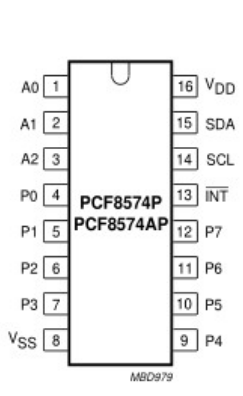
\includegraphics[width=0.3\textwidth]{pcf.png}
    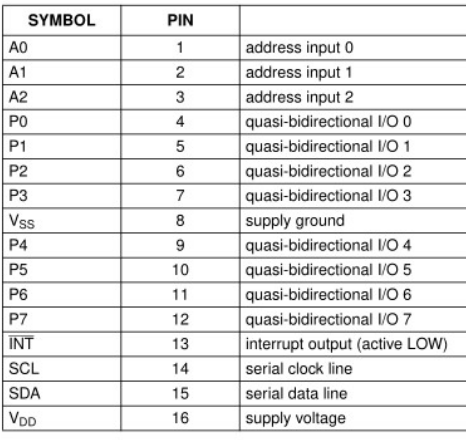
\includegraphics[width=0.4\textwidth]{pcf-pins.png}
    \caption{PCF8574}
\end{figure}

\begin{itemize}
    \item Er zijn 2 types van de PCF8574:
    \begin{enumerate}
        \item PCF8574 met vast adres 32 (0x020)
        \item PCF8574A met vast adres 56 (0x38)
    \end{enumerate}
\end{itemize}

\begin{figure}[H]
    \centering
    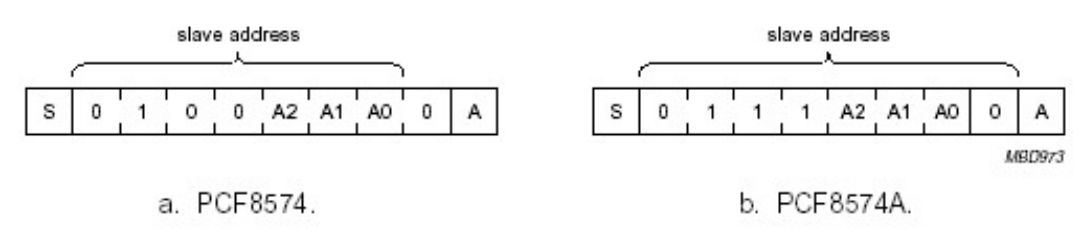
\includegraphics[width=0.6\textwidth]{pcf-adres.png}
    \caption{PCF8574 en PCF8574A adressen. A0, A1 en A2 kunnen we instellen door ze aan + of GND te hangen.}
\end{figure}

\subsection{Schakeling}

\begin{figure}[H]
    \centering
    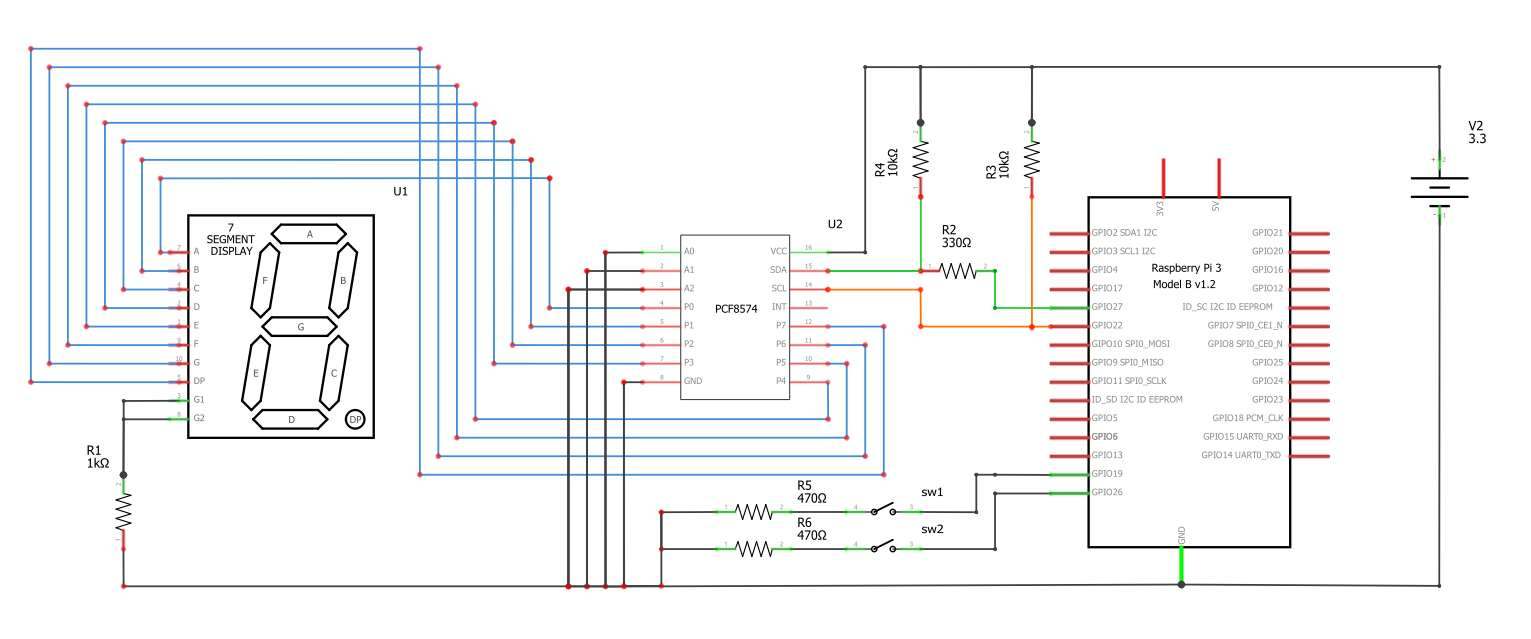
\includegraphics[width=\textwidth]{pcf-schakeling.png}
    \caption{PCF8574 met 7-segment display}
\end{figure}


\section{LCD Display}

\subsection{Pinconfiguratie}
\begin{figure}[H]
    \centering
    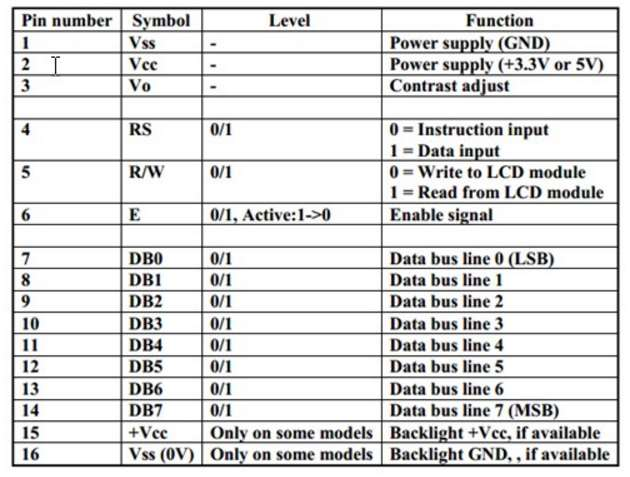
\includegraphics[width=0.6\textwidth]{lcd-pin.png}
    \caption{Pinconfiguratie LCD display}
\end{figure}

\subsection{Protocol LCD-displaycontroller (HD44780/KS0066)}
\begin{figure}[H]
    \centering
    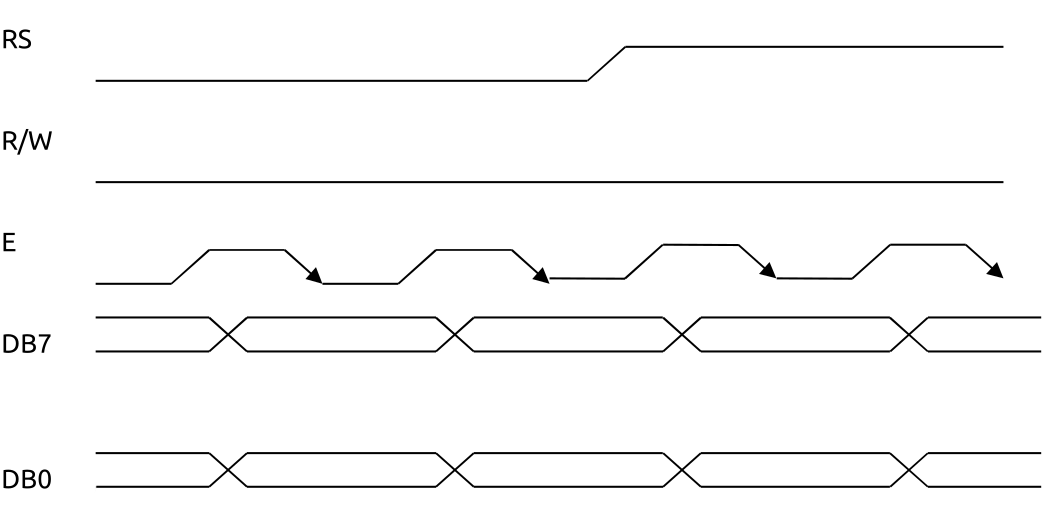
\includegraphics[width=0.5\textwidth]{lcd-timing.png}
    \caption{Timingdiagram LCD}
\end{figure}

\begin{itemize}
    \item Het enable signaal E kunnen we vergelijken met het kloksignaal SCL van de SPI-bus of het shiftregister
    \item Per klokpuls (in tegenstelling tot de voorbije hoofdstukken: bij de dalende flank) worden 8 bits data verwerkt
    \item De volgorde van de signalen is heel belangrijk:
    \begin{enumerate}
        \item Enable hoog
        \item Data klaarzetten
        \item Enable laag
        \item delay
        \item \dots
    \end{enumerate}
    \item Er zijn nog 2 controlelijnen:
    \begin{enumerate}
        \item R/W bepaalt of we data lezen of schrijven (0=schrijven, 1=lezen)
        \item RS (register select): bepaalt of een instructie of character wordt gestuurd. 
    \end{enumerate}
\end{itemize}

\subsection{Schakeling}

\begin{figure}[H]
    \centering
    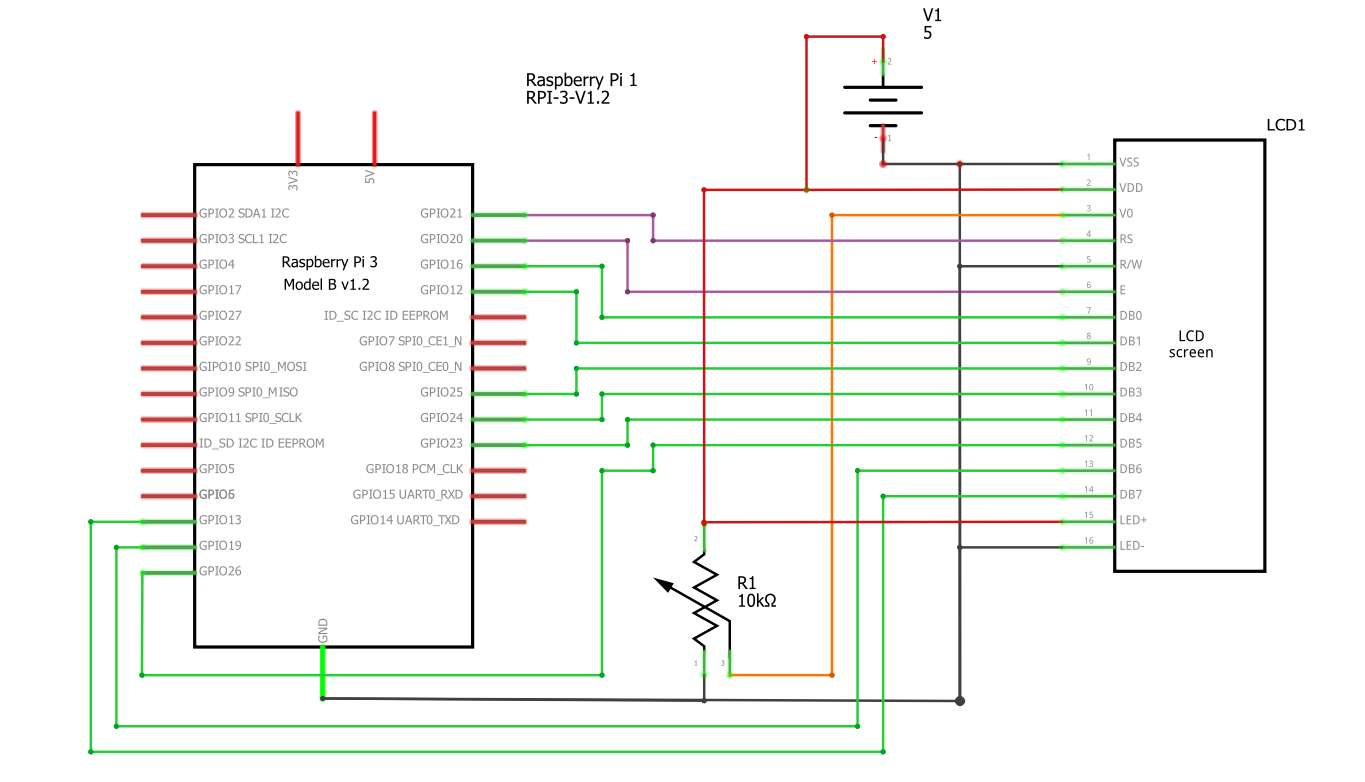
\includegraphics[width=\textwidth]{lcd.png}
    \caption{LCD schakeling}
\end{figure}


\subsection{Basisinstructies}
\begin{figure}[H]
    \centering
    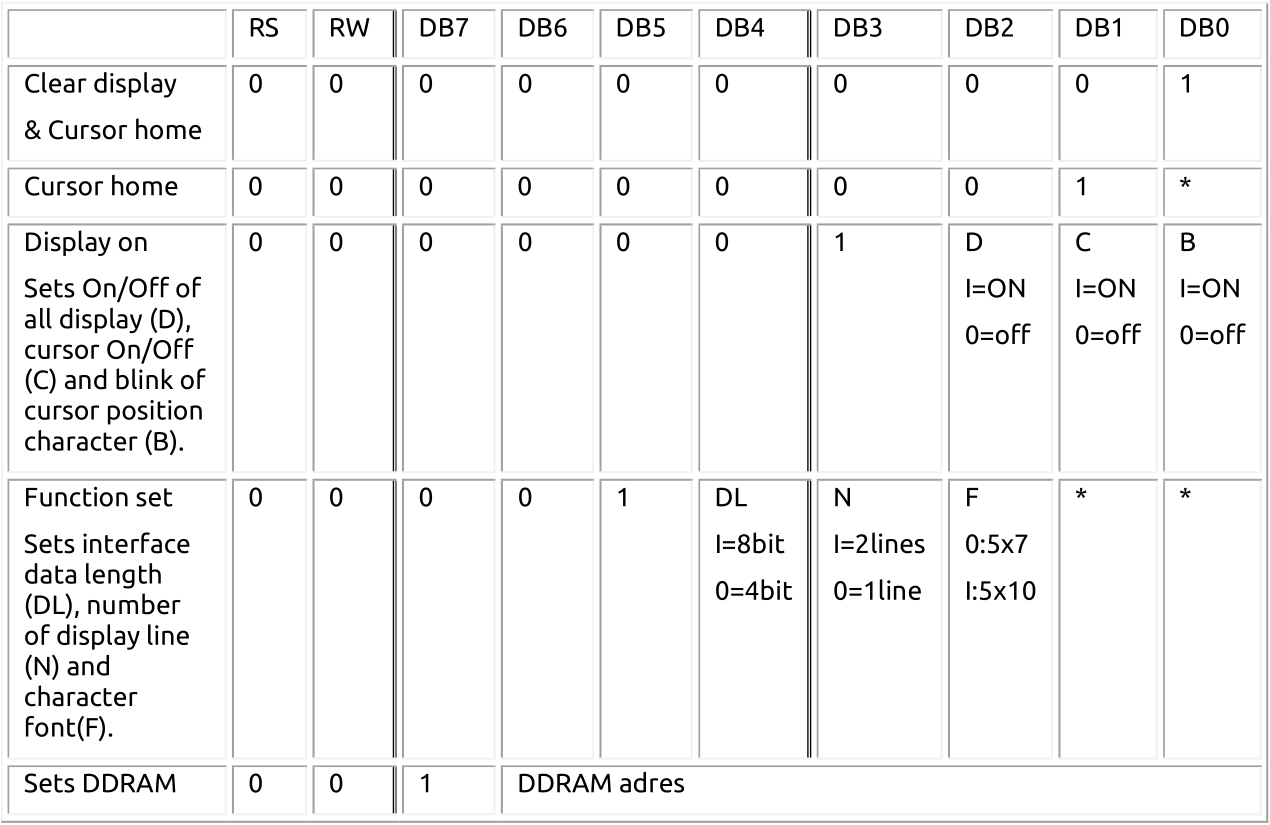
\includegraphics[width=0.65\textwidth]{lcd-instructies.png}
    \caption{Basisinstructies LCD controller}
\end{figure}

Om het display te initialiseren moeten we volgende instructies aanroepen:
\begin{itemize}
    \item Function set (met type display: 2 lijnen, karakters = 5x7 pixels, datalengte = 8bit)
    \item Display on
    \item Clear display en cursor home
\end{itemize}


\subsection{Geheugen adressen van het LCD display}
De controller van het display kan ook een display aansturen van 4x20 karakters, 
daarom beschikt de controller over 40 geheugenadressen. 

\begin{itemize}
    \item Eerste lijn: adressen 0x00 t.e.m. 0x0F
    \item Tweede lijn: adressen 0x40 t.e.m. 0x4F
\end{itemize}

\section{MPU 6050}

= chip die op de GY-521 module zit in onze kit. 

\begin{itemize}
    \item De module kan:
    \begin{itemize}
        \item versnelling meten
        \item orientatie bepalen
        \item temperatuur meten
    \end{itemize}
    \item De metingen worden gedigitaliseerd met een 16-bit ADC 
    \item Het bereik kan worden ingesteld (2-16g voor de accelerometer, 250-200°/s voor de gyroscoop)
    \item Je kan de chip laten detecteren wanneer hij in vrije val is en daarop een interrupt-signaal laten genereren op de voorziene pin.
\end{itemize}

\subsection{Schakeling}
\begin{figure}[H]
    \centering
    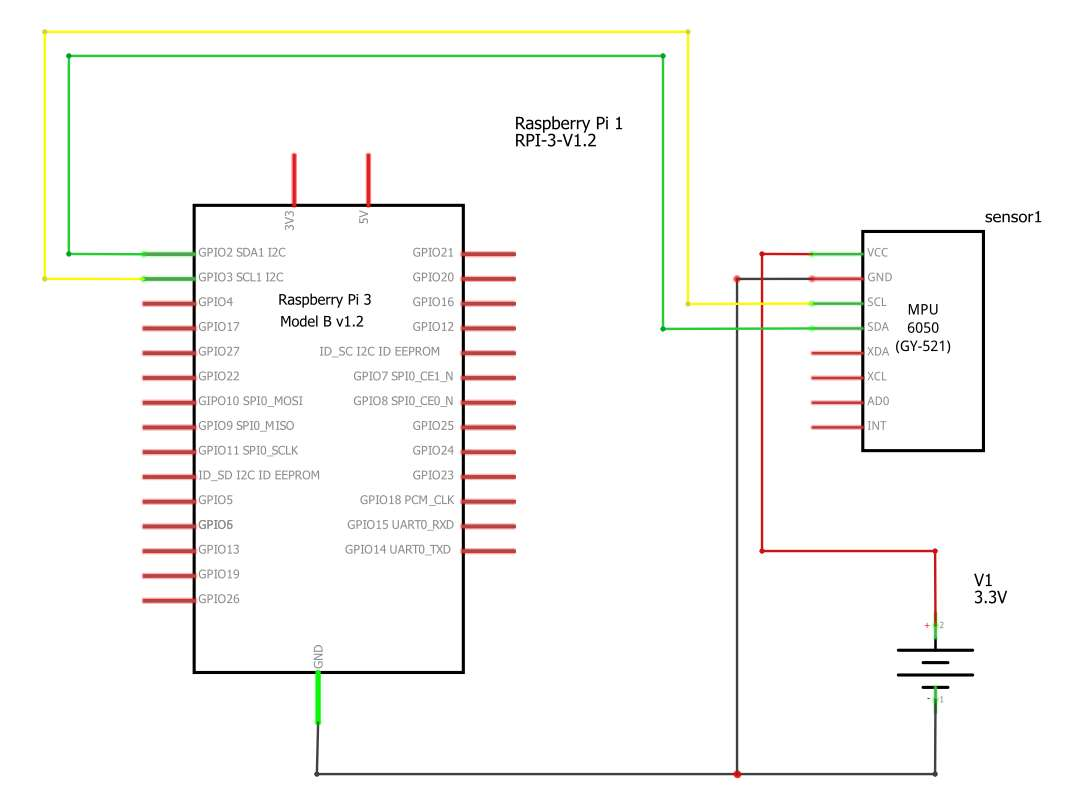
\includegraphics[width=0.9\textwidth]{mpu6050.png}
    \caption{MPU6050 schakeling met Raspberry Pi}
\end{figure}




\subsection{Meetresultaten inlezen}

\begin{itemize}
    \item Kan via:
    \begin{itemize}
        \item SPI
        \item $\text{I}^2\text{C}$
    \end{itemize}
    \item De GY-521 module werkt van 2.0 t.e.m. 3.6V (dus voeden met 3.3V van externe voeding)
    \item De MPU6050 digitaliseert de metingen met een 16-bit ADC, elke waarde neemt dus 2 registers in beslag en wordt in big-endian formaat opgeslagen
\end{itemize}



\subsection{SM-bus (System Management Bus)}
= interface gebaseerd op $\text{I}^2\text{C}$, met o.a. strikte paramters voor timing en voltage en een aantal vaste transacties.

De bus zal zelf zorgen voor start- en stopconditie, acknowledges, en versturen van data. 
We moeten enkel nog de correct instructie aanroepen, het adres meegeven, de eventuele data klaarzetten of inlezen.

\subsection{Inertial Measurement Unit (IMU)}
= een module om beweging en/of orientatie in 3D te bepalen. 
Daarvoor wordt gebruik gemaakt van 1 of meer sensoren die telkens een resultaat voor de 3 assen (x,y,z) geven.

\begin{itemize}
    \item Wordt gebruikt in smartphones, vlieg- en ruimtetuigen, game controllers, \dots
    \item IMU's worden ingedeeld volgens het aantal \textit{degrees of freedom} (DOF):
    een accelerometer heeft 3 assen, als je een gyroscoop aan toevoegt heb je 6-DOF IMU, + magnetometer = 9-DOF IMU.
    \item Deze sensoren zijn \textit{Micro Electro-Mechanical Systems (MEMS)} die werken met miniscule mechanische componenten op een chip.
\end{itemize}

\subsection{Accelerometer}
\begin{itemize}
    \item Meet versnelling (= verandering van beweging) in 3 dimensies
    \item Eenheid: $\text{m/s}^2$ of g-force
    \item Bestaat uit:
    \begin{itemize}
        \item een aantal vaste platen
        \item daartussen een bewegende massa die is opgehangen aan een veersysteem
    \end{itemize}
    \item De vaste plaat en bewegende massa vormen een condensator waardoor de capaciteit door de sensor kan worden gemeten
    \item Een accelerometer bevat 3 zulke opstellingen, 1 voor elke dimensie
\end{itemize}

\begin{figure}[H]
    \centering
    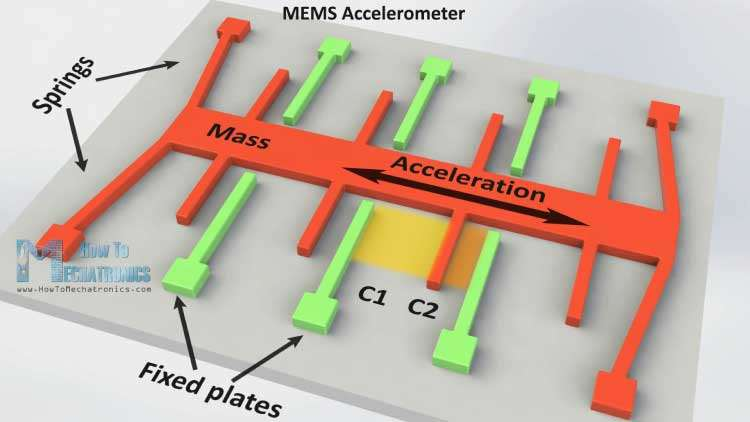
\includegraphics[width=0.4\textwidth]{accelerometer.png}
    \caption{Accelerometer}
\end{figure}


\subsection{Gyroscoop}
\begin{itemize}
    \item Meet hoeksnelheid of veranderingen in orientatiehoek in 3 dimensies
    \item Eenheid: $\degree$/s
    \item Werkt zoals de accelerometer, maar dan met een massa die kan draaien ipv schuiven.
    \item Als de beginorientatie bekend is, kan je door continu de veranderin erbij te tellen ook de huidige orientatie bepalen
\end{itemize}

\begin{figure}[H]
    \centering
    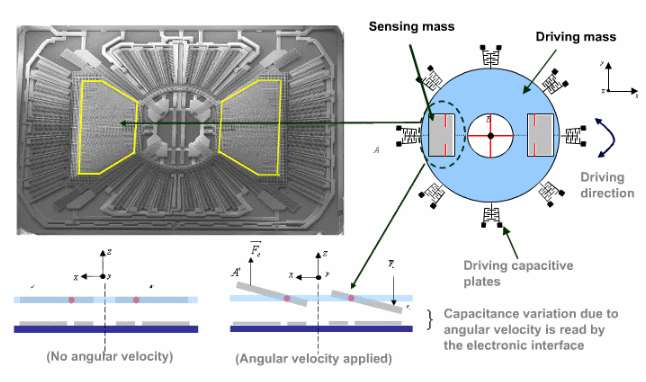
\includegraphics[width=0.6\textwidth]{gyroscope.png}
    \caption{Gyroscoop}
\end{figure}


\subsection{Magnetometer}
\begin{itemize}
    \item Meet de sterkte van het magnetisch veld in 3 richtingen
    \item Eenheid: Tesla (meestal micro- of nano-)
    \item Met een magnetometer kunnen we dus een kompas toevoegen aan de meting en wordt het geheel nog een stuk betrouwbaarder
\end{itemize}


\subsection{Registers}
De MPU6050 heeft veel registers. Elk register heeft een bepaalde functie.

\begin{itemize}
    \item Power management: 0x6B
    \item Accelerometer configuratie: 0x1C
    \item Accelerometer metingen: in te lezen via registers 0x3B t.e.m. 0x40
    \item Gyroscoop configuratie: 0x1B
    \item Gyroscoop metingen: in te lezen via registers 0x43 t.e.m. 0x48
    \item Temperatuur metingen: in te lezen op registers 0x41 en 0x42
\end{itemize}

\section{Rotary encoder}
= een soort draaibare knop

\begin{itemize}
    \item We kunnen uitlezen of we naar links of rechts draaien
    \item Geen begin of eindpositie (`zotte knop')
    \item Met tandjes: plaatjes in de stand waar de knop een stabiele positie heeft
\end{itemize}

\subsection{Werking}

\begin{itemize}
    \item Gemeenschappelijke ingang die verbonden is met een aantal contactzones op een schijf die met de knop meedraait.
    \item Twee uitgangen die verbonden zijn op een vast punt, met een kleine afstand ertussen.
    \item Drukknop
\end{itemize}

\begin{figure}[H]
    \centering
    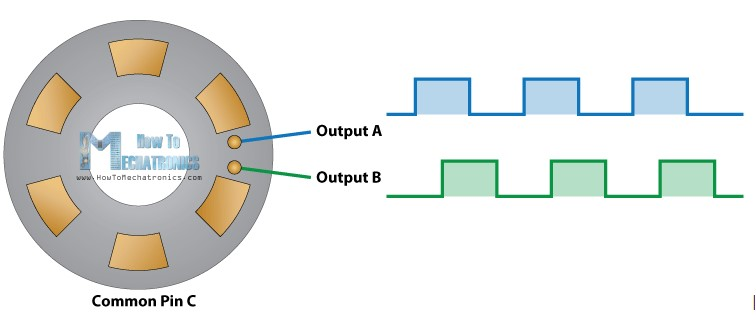
\includegraphics[width=0.5\textwidth]{rotary.png}
    \caption{Rotary encoder binnenkant}
\end{figure}

\begin{itemize}
    \item Telkens je de knop een tand verder draait, schuift een contactzone over de pinnen en maken ze even contact
    \item Naargelang de richtinv verschilt de volgorde
    \begin{itemize}
        \item In wijzerzin: eerst A, dan B
        \item In tegenwijzerzin: eerst B, dan A
    \end{itemize}
    \item Als je de ingang hoog trekt et een pull-up en aan de knop draait, krijg je op beide uitgangen een blokgolf:
\end{itemize}

\begin{figure}[H]
    \centering
    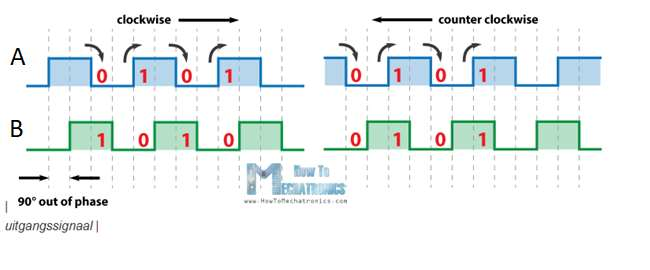
\includegraphics[width=0.6\textwidth]{rotary-werking.png}
    \caption{Rotary encoder: wijzerzin/tegenwijzerzin}
\end{figure}

\subsection{Pinconfiguratie}

\begin{figure}[H]
    \centering
    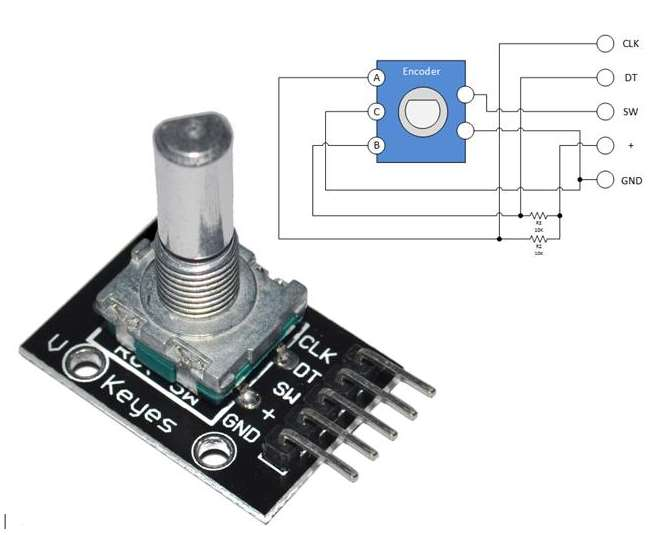
\includegraphics[width=0.5\textwidth]{rotary-pins.png}
    \caption{Pinconfiguratie rotary encoder}
\end{figure}

\begin{itemize}
    \item A, B, C zijn respectievelijk de CLK, DT en GND pin
    \item De rechteruitgangen zijn uitgangen voor de knop, gaat naar SW en GND (nog een pull-up nodig)
    \item De + moet verbonden zijn met 3.3V: zorgt voor de pull-upfunctie van de encoder.
\end{itemize}

\section{MAX7219 serial interfaced, 8-digit display driver}
= een driver-IC voor het aansturen van maximaal 8 7-segementdisplays via SPI. 

\begin{itemize}
    \item De chip heeft 8 registers die telkens ofwel een BCD-encoded cijfer of een 8-bitwaarde kunnen opnemen
    \item Het decoderen van BCD en multiplexen van de 8 displays doet de chip volledig zelf.
\end{itemize}

\subsection{Pinconfiguratie}
\begin{figure}[H]
    \centering
    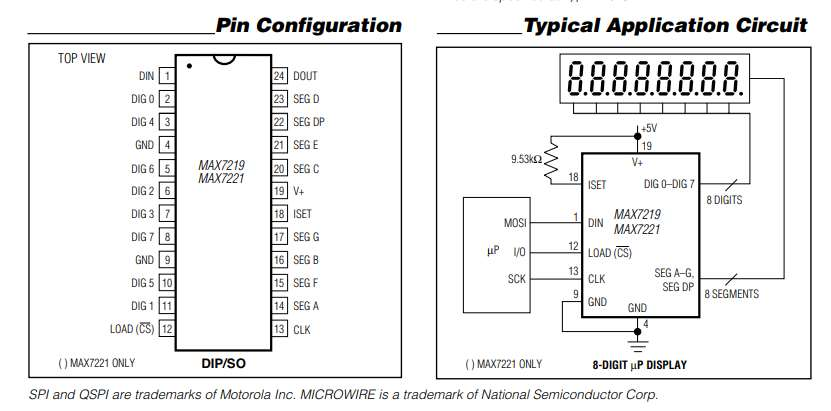
\includegraphics[width=0.75\textwidth]{max7219-pins.png}
    \caption{Pinconfiguratie MAX7219}
\end{figure}

We gebruiken deze chip voor het aansturen van een 8x8 LED-matrix:

\begin{figure}[H]
    \centering
    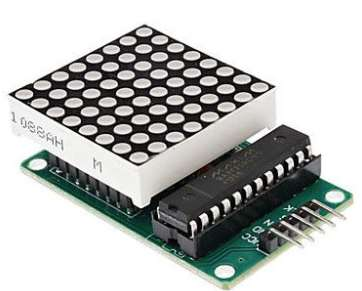
\includegraphics[width=0.4\textwidth]{matrix.png}
    \caption{MAX7219 LED Matrix Module}
\end{figure}

\subsection{Schakeling}

Deze module heeft maar naast voeding en massa slechts 3 aansluitingen ipv de gebruikelijke 4 voor SPI:
de MISO-pin is niet nodig want er kan toch niet geschreven worden naar de registers van de MAX7219.

Verbind de MAX7219/led matrix met de SPI bus van RPi en de 5V voeding van de externe
voeding. We mogen de stuursignalen direct tussen de RPi en het bordje verbinden (zonder
level shifter), gezien we vanuit de 3,3 volt de 5 volt aansturen, en er niets terug komt.


\subsection{Registers}
De MAX7219 beschikt over 14 registers:

\begin{table}[H]
    \centering
    \begin{tabular}{|l|l|}
        \hline
        \multicolumn{1}{|c|}{\textbf{Register}} & \multicolumn{1}{c|}{\textbf{Functie}}                                                                                                          \\ \hline
        0x80                                    & \begin{tabular}[c]{@{}l@{}}No-Op(eration) register, enkel nodig wanneer \\ je meerdere modules achter elkaar hangt\end{tabular}                \\ \hline
        0x1-0x8                                 & de data voor de 8 cijfers                                                                                                                      \\ \hline
        0x9                                     & Decode mode: om met BCD's te kunnen werken                                                                                                     \\ \hline
        0xA                                     & Intensity = helderheid, in 16 stappen (van 0x0 tot 0xF)                                                                                        \\ \hline
        0xB                                     & \begin{tabular}[c]{@{}l@{}}Scan Limit: stelt in hoeveel cijfers er zijn aangesloten \\ (bij ons: 7, want de matrix heeft 8 rijen)\end{tabular} \\ \hline
        0xC                                     & Shutdown: 1 als LSB om de uitgangen te activeren                                                                                               \\ \hline
        0xF                                     & Display test: alle LEDs oplichten                                                                                                              \\ \hline
    \end{tabular}
\end{table}

\subsection{Gebruik in Python}

\begin{lstlisting}[language=Python]
from spidev import SpiDev
spi = SpiDev()

# Bus is 0, device is de gekozen CE-pin (0 of 1)
spi.open(bus, device)                

# Klokfrequentie instellen (hier: 100kHz)
spi.max_speed_hz = ...                  

# Waarde naar register schrijven
spi.writebytes([register, value])       
\end{lstlisting}



\end{document}
